%%
%% 研究報告用スイッチ
%% [techrep]
%%
%% 欧文表記無しのスイッチ(etitle,eabstractは任意)
%% [noauthor]
%%

%\documentclass[submit,techrep]{ipsj}
%%% <<< SES
%\documentclass[submit,techrep,noauthor]{ipsj}
\documentclass[submit,ses,noauthor]{ipsj}
%%% >>> SES

\usepackage[dvipdfmx]{graphicx}
%\usepackage[dvips]{graphicx}
\usepackage{latexsym}
\usepackage[dvipdfmx,table,xcdraw]{xcolor}
\usepackage[T1]{fontenc}
\usepackage{lmodern}
\usepackage{textcomp}
\usepackage[hyphens]{url}
\usepackage[noadjust]{cite}
%\usepackage[fleqn]{amsmath}
%\usepackage{amssymb}
\usepackage{listings,jvlisting} %日本語のコメントアウトをする場合jvlisting(もしくはjlisting)が必要
\usepackage{color}
\usepackage{booktabs}
\usepackage{indentfirst}


%ここからソースコードの表示に関する設定
\newcommand{\listingcaption}[1]{
\refstepcounter{lstlisting}
\smallskip
\centerline{
Listing \thelstlisting\quad#1
\vspace{-1mm}
}}

\definecolor{darkgray}{rgb}{.4,.4,.4}
\definecolor{purple}{rgb}{0.65, 0.12, 0.82}

\lstdefinelanguage{JavaScript}{
  keywords={typeof, new, true, false, catch, function, return, null, catch, switch, var, if, in, while, do, else, case, break},
  keywordstyle=\color{blue}\bfseries,
  ndkeywords={class, export, boolean, throw, implements, import, this},
  ndkeywordstyle=\color{darkgray}\bfseries,
  identifierstyle=\color{black},
  sensitive=false,
  comment=[l]{//},
  morecomment=[s]{/*}{*/},
  commentstyle=\color{purple}\ttfamily,
  stringstyle=\color{red}\ttfamily,
  morestring=[b]',
  morestring=[b]"
}

\lstset{
  basicstyle={\ttfamily},
  identifierstyle={\small},
  commentstyle={\smallitshape},
  keywordstyle={\small\bfseries},
  ndkeywordstyle={\small},
  stringstyle={\small\ttfamily},
  frame={tb},
  breaklines=true,
  columns=[l]{fullflexible},
  numbers=left,
  language=JavaScript,
  keywordstyle={\small\bfseries \color[rgb]{1,0,0}},
  xrightmargin=0zw,
  xleftmargin=3zw,
  numberstyle={\scriptsize},
  stepnumber=1,
  numbersep=1zw,
  lineskip=-0.5ex
}
%ここまでソースコードの表示に関する設定


\newcommand{\todo}[1]{\colorbox{yellow}{{\bf TODO}:}{\color{red} {\textbf{[#1]}}}}

\def\Underline{\setbox0\hbox\bgroup\let\\\endUnderline}
\def\endUnderline{\vphantom{y}\egroup\smash{\underline{\box0}}\\}
\def\|{\verb|}
%

%\setcounter{巻数}{59}%vol59=2018
%\setcounter{号数}{10}
%\setcounter{page}{1}


\begin{document}


\title{情報処理学会研究報告の準備方法\\
(2018年10月29日版)}

\etitle{How to Prepare Your Paper for IPSJ SIG Technical Report \\ (version 2018/10/29)}

\affiliate{WA}{和歌山大学\\
Faculty of Systems Engineering, Wakayama University, 30 Sakaedani, Wakayama, 640--8441 Japan}


\paffiliate{NAIST}{奈良先端科学技術大学院大学\\
Nara Institute of Science and Technology, 8916--5 Takayama-cho, Ikoma, Nara, 630--0192 Japan}

\author{大森 楓己}{Omori Fuki}{WA}[s246328@wakayama-u.ac.jp]
\author{伊原 彰紀}{Ihara Akinori}{WA}[ihara@wakayama-u.ac.jp]
\author{柏 祐太郎}{Kashiwa Yutaro}{NAIST}[yutaro.kashiwa@is.naist.jp]


\begin{abstract}
\todo{SSのまま}プログラムには同じ機能を実現する実装方法が複数存在し,それぞれ実行速度が異なる.大規模なプログラムの各機能において手動で実装方法を検討することは困難である.本研究では,部分的なプログラムの実行速度を計測するマイクロベンチマーク共有サービスMeasureThat.netから収集した評価結果を学習データセットとしたニューラル機械翻訳モデルを用いて実行速度の改善に特化したプログラム自動修正モデルを構築した.
\end{abstract}


%
%\begin{jkeyword}
%情報処理学会論文誌ジャーナル,\LaTeX,スタイルファイル,べからず集
%\end{jkeyword}
%
%\begin{eabstract}
%This document is a guide to prepare a draft for submitting to IPSJ
%Journal, and the final camera-ready manuscript of a paper to appear in
%IPSJ Journal, using {\LaTeX} and special style files.  Since this
%document itself is produced with the style files, it will help you to
%refer its source file which is distributed with the style files.
%\end{eabstract}
%
%\begin{ekeyword}
%IPSJ Journal, \LaTeX, style files, ``Dos and Dont's'' list
%\end{ekeyword}

\maketitle

%%%%%%%%%%%%%%%%
\section{はじめに}
%%%%%%%%%%%%%%%%

Webアプリケーションでは,読み込み時間が10秒のWebページは1秒のページと比較してユーザの離脱率が123\%増加する\cite{an_2018}など,実行速度はソフトウェア品質に直結する重要な要素である.実行速度に影響を与える要因のひとつがプログラム実装方法である.プログラムに使用するAPIやアルゴリズムの違いによって同じ機能を実現する実装方法が複数存在する.Webアプリケーションの代表的な開発言語であるJavaScriptでは,初回実行時に実行時(Just-In-Time; JIT)コンパイラによってプログラムをコンパイルし,以後の実行を高速化するが,JITコンパイラによっては最適化が十分でなく開発者の実装方法によってコンパイル後のオブジェクトコードが異なるため,実行速度に差が生じる.

ソフトウェア開発者は,アプリケーションの部分的なプログラムの実行速度を計測するマイクロベンチマークを用いて複数の実装方法を比較し,高速な実装方法を把握できる.マイクロベンチマーク共有サービスMeasureThat.netでは,開発者が計測に用いたマイクロベンチマークを他開発者に共有することで,高速な実装方法の情報交換が行われている.しかし,MeasureThat.net上に投稿された膨大なマイクロベンチマークの中から,機能に応じた高速な実装方法を手動で把握することは困難である.

本研究では,MeasureThat.net\footnote{\url{https://www.measurethat.net/}}から収集した実行速度の計測結果を学習データセットとして活用した,実行速度改善のためのプログラム自動修正モデルを作成する.プログラム自動修正は,主にプログラムの実行時エラーを修正するための手法として従来から研究されており,開発者によるエラー修正パッチのパターンなどが調査されている.近年では,自然言語間の翻訳タスクに用いられていたニューラル機械翻訳を用いて修正パッチを生成する手法が複数提案されている\cite{lutellier_2020}.ニューラル機械翻訳を用いた手法ではバグを含む行の前後の命令を入力に含み,他手法に比べて文脈に応じた修正パッチを柔軟に生成することができる.特に,言語設計上の事由で静的解析が困難なJavaScript等の言語においても他手法を上回る修正性能が報告されているため\cite{lutellier_2020},本研究でもプログラム自動修正にニューラル機械翻訳を用いる.

本研究では,実行時エラーの修正を目的とした従来のプログラム自動修正手法を転用し,マイクロベンチマーク共有サービスMeasureThat.netから収集した実行速度の計測結果を学習データセットとしたニューラル機械翻訳モデルを用いて,実行速度改善における自動修正の効果を明らかにする.モデルの評価のため,GitHubにおけるスター数上位のJavaScriptプロジェクトを対象に高速化修正パッチの自動生成を試み,修正パッチのテスト通過率と実行速度の改善度を調査する.

本論文では,\ref{sec:back}章でプログラム実行速度の改善に関する従来研究,\ref{sec:approach}章でニューラル機械翻訳モデルの学習方法について述べる.そして\ref{sec:pre}章では事前実験,\ref{sec:evaluation}章では実装モデルの評価実験手順について述べる.\ref{sec:discussion}章では評価実験をもとに提案手法についての考察を述べる.最後に\ref{sec:conclusion}章でまとめを述べる.


%%%%%%%%%%%%%%%%%%%
\section{プログラム実行速度の改善}\label{sec:back}
%%%%%%%%%%%%%%%%%%%

\subsection{プログラム実行速度改善の試み}

プログラム実行速度は,ソフトウェア品質に直結する重要な要素である.実行速度を改善する研究として,Xuは著者が特定したUML設計モデルの修正ルールに基づいたWebアプリケーションの設計工程における自動ボトルネック修正手法を提案している\cite{xu_2008}.また,実装工程での速度改善支援として,Selakovicらはパフォーマンス問題の主な原因が非効率的なAPIの使用であり,またほとんどの問題は数行のコード最適化によって解決されることを明らかにした一方で,JavaScriptの言語設計上,ルールベース自動修正手法では変数の型や式の値の静的解析が困難であることを明らかにした\cite{selakovic_2016}.Saikiらは開発者による手動最適化支援のためマイクロベンチマーク共有サービスjsPerfに投稿されたプログラムの機能ごとの分類手法を提案している\cite{saiki_2021}.
本研究では,実行速度に影響を与える要因のひとつであるプログラム実装方法に注目し,実装工程での実行速度自動改善を目指す.

\subsection{マイクロベンチマークを用いた実行速度の比較}

マイクロベンチマークは,ソフトウェアの部分的なプログラムの実行速度を計測するために用いられる検証用のプログラムである.ソフトウェア開発者は,マイクロベンチマークを用いて複数の実装方法を比較し,高速な実装方法を把握できる.マイクロベンチマーク共有サービスMeasureThat.netでは,開発者が計測に用いたマイクロベンチマークを他開発者に共有することで,高速な実装方法の情報交換が行われている.MeasureThat.netはJavaScriptプログラムの実行速度をブラウザ上で比較できるほか,比較したプログラムセットはMeasureThat.net上に記録・公開され,他者のプログラムセットを自由に閲覧できる.

%\begin{figure}[t]
%\centering
%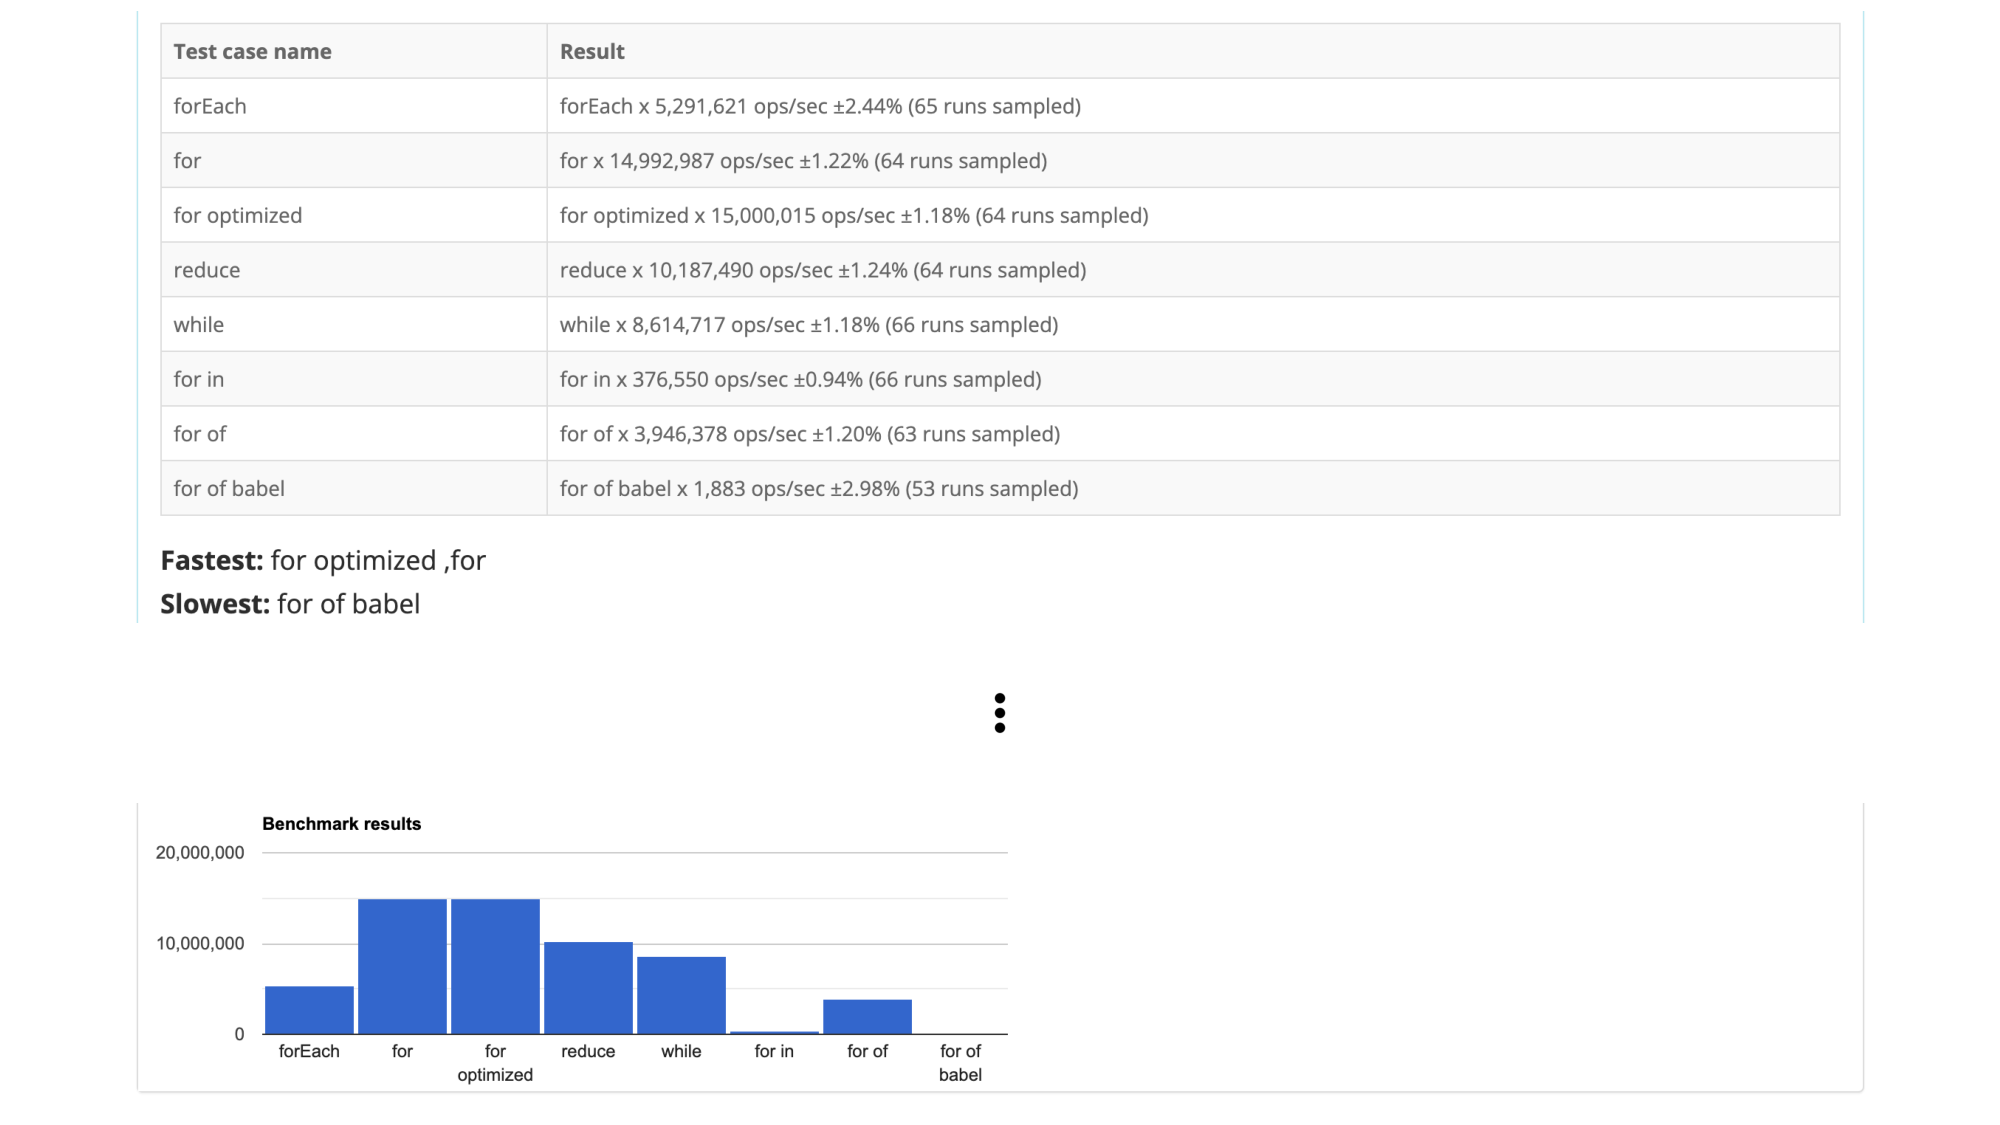
\includegraphics[width=0.95\linewidth]{figure/measureThat.pdf}
%\caption{measureThat.netによる実行速度計測}
%\label{figure:measureThat}
%\end{figure}

MeasureThat.netに投稿されるマイクロベンチマークは,実行速度の計測前に共通して行う事前処理を記述する事前処理コードと,同じ機能を実現する複数のプログラム群からなる.MeasureThat.netで評価された配列testDataの要素の総和を計算するプログラム\footnote{\url{https://www.measurethat.net/Benchmarks/Show/10352/0/foreach-vs-for-len-vs-for-in-vs-for-of-vs-babel-for-of}}では,8パターンの実装方法を比較している.表\ref{table:speed}は,実行速度の違いを示す.最も高速な実装方法はfor optimizedであり,for of babelの約8,000倍の実行速度であった.その他にfor,for optimized,for of babelはすべてfor文を用いており,特にfor of babelは命令数が比較的多いために実行速度が低いと考えられる.また,APIの呼出しは実行速度低下の要因である\cite{selakovic_2016}ため,for optimizedはforに比べてプロパティlengthの呼出し回数が少ないことで速度が向上したと考えられる.この事例のように,実装方法により実行速度は異なるため,本研究では,マイクロベンチマーク共有サービスMeasureThat.netから収集した実行速度の計測結果を学習データセットとして活用した,実行速度改善のためのプログラム自動修正手法を提案する.


\begin{table}[t]
  \caption{プログラム実行速度}
  \label{table:speed}
  \centering
    \scalebox{0.9}[0.9]{
  \begin{tabular}{c|r}
    \hline
    プログラム & 実行速度[ops/sec]\\
    \hline
    forEach & 5,291,621 \\
    for & 14,992,987 \\
    for optimized & 15,000,015 \\
    reduce & 10,187,490 \\
    while & 8,614,717 \\
    for in & 376,550 \\
    for of & 3,946,378 \\
    for of babel & 1,883 \\
    \hline
  \end{tabular}
  }
  \vspace{-4mm}
\end{table}

%
%
%\listingcaption{事前処理コード}
%\begin{lstlisting}[label=list:preparation]
%var testData = [];
%for (var i = 0; i < 100; i++) {
%  testData.push(i);
%}
%\end{lstlisting}
%
%プログラム\ref{list:preparation}は,配列testDataを宣言し,testDataの要素に0〜99の整数を追加する.プログラム\ref{list:forEach}〜\ref{list:for of babel}は,すべてプログラム\ref{list:preparation}で作成されたtestDataの要素の総和を算出するプログラムである.
%
%\listingcaption{forEach}
%\begin{lstlisting}[label=list:forEach]
%var res = 0;
%testData.forEach(function(x) {
%  res += x;
%});
%\end{lstlisting}
%
%プログラム\ref{list:forEach}は,forEach()メソッドを用いて総和を算出する.forEach()メソッドは,与えられるコールバック関数を配列の各要素に対して一度ずつ実行するメソッドである.
%
%\listingcaption{for}
%\begin{lstlisting}[label=list:for]
%var res = 0;
%for (var i = 0; i < testData.length; i++) {
%  res += testData[i];
%}
%\end{lstlisting}
%
%プログラム\ref{list:for}は,for文を用いて総和を算出する.
%
%\listingcaption{for optimized}
%\begin{lstlisting}[label=list:for optimized]
%var res = 0;
%for (var i = 0, len = testData.length; i < len; i++) {
%  res += testData[i];
%}
%\end{lstlisting}
%
%プログラム\ref{list:for optimized}はプログラム\ref{list:for}と同様にfor文を用いているが,testDataのlengthプロパティをループの度に参照する代わりに変数lenを用いる.
%
%\listingcaption{reduce}
%\begin{lstlisting}[label=list:reduce]
%var res = testData.reduce(function(sum, x) {
%  return sum + x;
%}, 0);
%\end{lstlisting}
%
%プログラム\ref{list:reduce}はreduceメソッドを用いて総和を算出する.reduce()メソッドは,与えられるコールバック関数を配列の各要素に対して一度ずつ実行するプログラムである.コールバック関数は,直前の要素に対してコールバック関数を実行した時のコールバック関数の戻り値を引数に受け取ることができ,最後の要素に対してのコールバック関数の戻り値が最終的なreduce()メソッドの戻り値となる.プログラム\ref{list:reduce}では,コールバック関数を用いて自身よりインデックスの小さい要素の総和を引数に受け取ることで最終的に全要素の総和を算出している.
%
%\listingcaption{while}
%\begin{lstlisting}[label=list:while]
%var res = 0;
%var i = testData.length;
%while (i--) {
%    res += testData[i];
%}
%\end{lstlisting}
%
%プログラム\ref{list:while}はwhile文を用いて総和を算出する.
%
%\listingcaption{for in}
%\begin{lstlisting}[label=list:for in]
%var res = 0;
%for (var data in testData) {
%  res += data;
%}
%\end{lstlisting}
%
%プログラム\ref{list:for in}はfor in文を用いて総和を算出する.for in文は連想配列等のキーが文字列であるオブジェクトに対して反復処理を行うための機能である.配列の反復に用いた場合,処理がインデックス順に行われないことがあるため,配列での使用は推奨されていない.
%
%\listingcaption{for of}
%\begin{lstlisting}[label=list:for of]
%var res = 0;
%for (var data of testData) {
%  res += data;
%}
%\end{lstlisting}
%
%プログラム\ref{list:for of}はfor of文を用いて総和を算出する.for of文は配列等の反復可能オブジェクトに対して反復処理を行うための機能である.
%
%
%\listingcaption{for of babel}
%\begin{lstlisting}[label=list:for of babel]
%var res = 0;
%var _iteratorNormalCompletion = true;
%var _didIteratorError = false;
%var _iteratorError = undefined;
%
%try {
%  for (var _iterator = testData[Symbol.iterator](), _step; !(_iteratorNormalCompletion = (_step = _iterator.next()).done); _iteratorNormalCompletion = true) {
%    var i = _step.value;
%  }
%} catch (err) {
%  _didIteratorError = true;
%  _iteratorError = err;
%} finally {
%  try {
%    res += testData[i];
%    if (!_iteratorNormalCompletion && _iterator.return) {
%      _iterator.return();
%    }
%  } finally {
%    if (_didIteratorError) {
%      throw _iteratorError;
%    }
%  }
%}
%\end{lstlisting}







\subsection{ニューラル機械翻訳を用いたプログラム自動修正}

部分的なプログラムの自動修正については,特に実行時エラーの修正を目的にこれまで多くの研究がされており,パターンマッチによる手法や遺伝的アルゴリズムを用いた手法などが提案されている.中でも近年では,ニューラル機械翻訳を用いたプログラム自動修正が複数提案されており\cite{chen_2018}\cite{lutellier_2020},言語設計上の事由で静的解析が困難なJavaScript等の言語においても他手法を上回る修正性能が評価されている\cite{lutellier_2020}.

ニューラル機械翻訳は,単語列を別の単語列に変換する深層学習モデルの一種であり,ニューラル機械翻訳を用いたバグ修正手法ではバグの前後の命令文を入力に含むことで,他手法に比べて文脈に応じた修正パッチを柔軟に生成することができる.

本研究では,実行時エラーの修正を目的とした従来のプログラム自動修正手法を転用し,MeasureThat.netから収集した実行速度の計測結果を学習データセットとしたニューラル機械翻訳モデルを用いて,実行速度改善における自動修正の効果を明らかにする.



\subsection{リサーチクエスチョン}

学習させたニューラル機械翻訳モデルによる修正性能を評価するため,2つのリサーチクエスチョンを設定する.

\noindent
\textbf{RQ1:生成パッチはどの程度テストを通過するか}

ニューラル機械翻訳モデルが生成する修正パッチは必ずしもJavaScriptの言語仕様に従うとは限らない.RQ1では入力プログラムと機能的に同一の処理を行うか確かめるため,どの程度テストスイートを通過するか明らかにする.

\noindent
\textbf{RQ2:生成パッチはどの程度実行速度を改善するか}

ニューラル機械翻訳モデルが生成する修正パッチを適用し,テストスイートを通過するプログラムが実行速度に与える効果について明らかにする.

%%%%%%%%%%%%%%%
\section{マイクロベンチマークを活用した実行速度改善}\label{sec:approach}
%%%%%%%%%%%%%%%

\subsection{手法概要}


本研究では,実行時エラーの修正を目的とした従来のプログラム自動修正手法CoCoNuT\cite{lutellier_2020}を転用し,MeasureThat.netから収集した実行速度の計測結果を学習データセットとした実行速度改善のためのニューラル機械翻訳モデルを作成する.

図\ref{figure:coconut}のように,CoCoNuTはプログラム行単位の修正を行うニューラル機械翻訳モデルであり,バグを含む行とその前後のプログラムを別個の畳み込みニューラルネットワークにより学習し,複数の修正パッチを出力する.また,異なる修正パターンに最適化された複数のモデルを用いるアンサンブル学習により,修正規模の異なるバグに柔軟に対応できる.CoCoNuTはJavaScriptを対象とする評価実験を行ったプログラム自動修正手法の中で筆者の調査した限り最新の研究であり,既存の他手法より修正性能に優れる.モデルの実装にはLutellierらの公開プログラム\footnote{\url{https://github.com/lin-tan/CoCoNut-Artifact}}を用いる.

\begin{figure}[t]
\centering
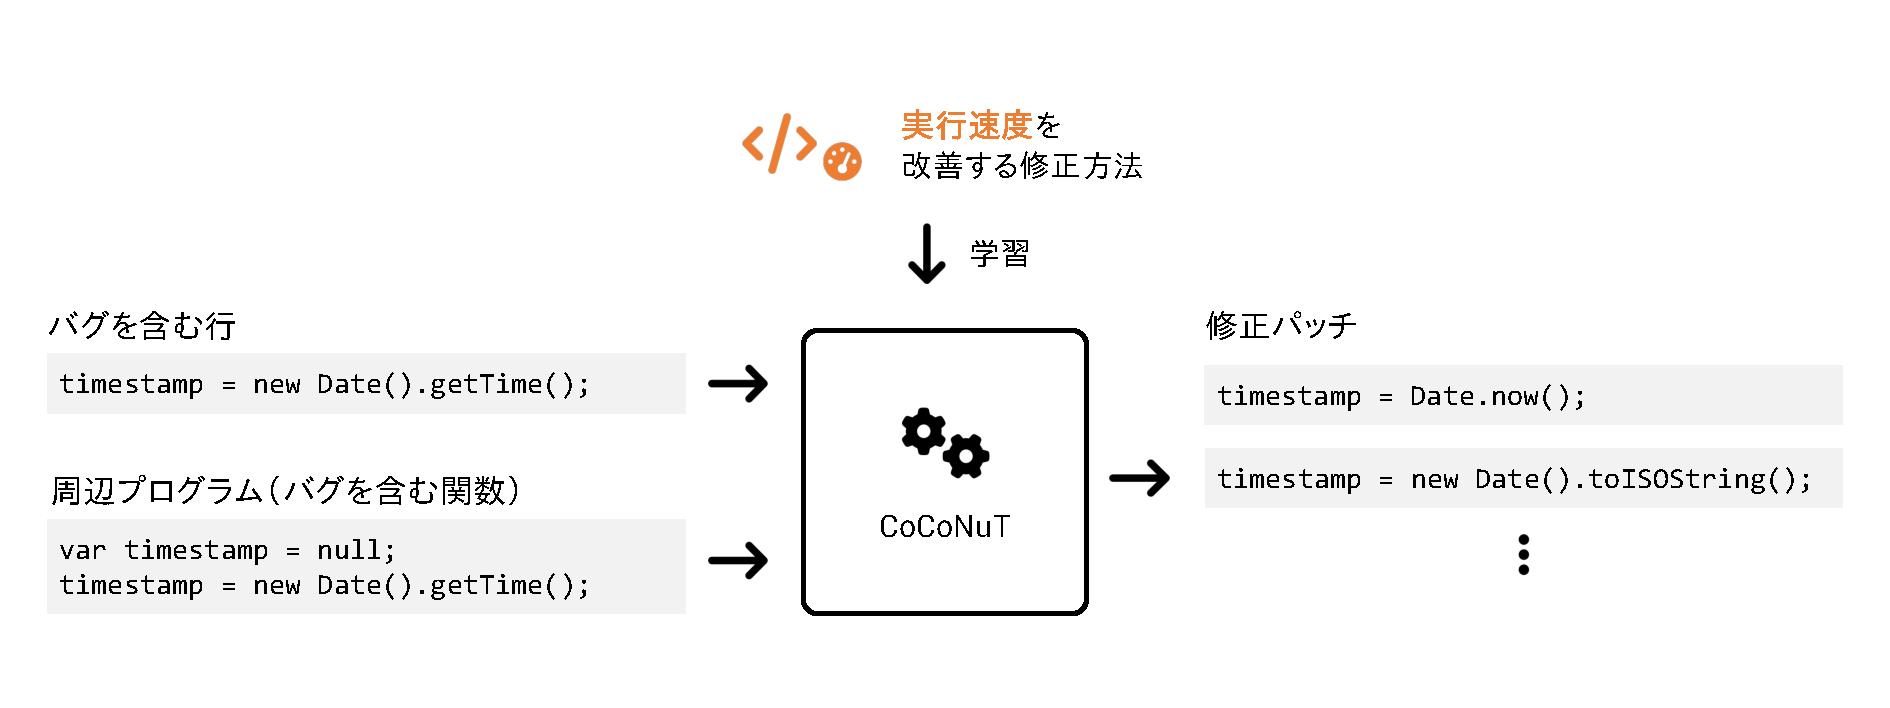
\includegraphics[width=0.95\linewidth]{figure/coconut.pdf}
\vspace{-4mm}
\caption{提案手法の概略図}
\vspace{-4mm}
\label{figure:coconut}
\end{figure}



\subsection{学習データセット}

学習データセットとして異なる方法で実装されたプログラム対を収集するため,まずMeasureThat.netから公開マイクロベンチマークを収集する.次に,収集した各マイクロベンチマークに対して実行速度を測定する.実行速度の計測にはBenchmark.jsライブラリ\footnote{\url{https://benchmarkjs.com/}}を用い,Chromeソフトウェア上でマイクロベンチマークを実行する.マイクロベンチマークが2件のプログラムを比較している場合,実行速度が速いプログラムを変更先プログラム,他方のプログラムを変更元プログラムとして双方の差分行を抽出し,プログラム対を作成する.また,マイクロベンチマークが3件以上のプログラムを比較している場合,最も実行速度が速いプログラムを変更先プログラム,他のプログラムを変更元プログラムとして各変更元プログラムと変更先プログラムの差分行を抽出し,複数のプログラム対を作成する.作成したプログラム対のうち,従来研究で提案されたモデルに入力可能な差分行が1行のみのプログラム対を学習データセットに用いる.その結果,8,144件のプログラム対を収集した.


\subsection{ニューラル機械翻訳モデルの学習}

前節で作成した学習データセットを用いてCoCoNuTの学習を行う.学習時のハイパーパラメータは公開プロジェクトに記述されている値を用い,バッチ数48,最大エポック数20に設定した.また,公開プログラムは「===」や「!==」等の一部演算子を正しくトークン化できていなかったため,当該箇所に修正を加えた.

%%%%%%%%%%%%%%%%%%%
\section{事前実験}\label{sec:pre}
%%%%%%%%%%%%%%%%%%%

本性では,自動修正モデルが高速な代替の実装方法を生成できるか検証する.

\subsection{実験方法}

学習データとして収集した8,144件のプログラム対からなる学習データセットを対象に10分割交差検証を行う.学習データセットを無作為に10グループに分割し,分割した各グループの変更元プログラム行に対して,他の9グループを統合した学習データセットを自動修正モデルに学習させ,実行速度修正パッチを生成する.そして,各グループ内で,自動修正モデルが変更先プログラム行に完全一致する修正パッチを生成できた割合を測定する.

\subsection{実験結果}

表\ref{table:preex}は,10分割交差検証の結果を示す.表中のヒューリスティックルール適用前に修正パッチの生成に成功した件数,失敗した件数,成功率を示す.学習データセットの6.94\%〜12.02\%のプログラムに対して,教師データに完全に一致する修正パッチを生成することができた.

%--------------------------
\begin{table}[t]
  \caption{事前実験結果}
  \label{table:preex}
  \centering
  \scalebox{0.8}[0.8]{
  \begin{tabular}{c|rrr|rrr}
    \hline
     & \multicolumn{3}{c|}{ヒューリスティックルール適用前} & \multicolumn{3}{c}{ヒューリスティックルール適用後} \\ \cline{2-7}
     & \multicolumn{1}{c}{生成} &  \multicolumn{1}{c}{生成} &  \multicolumn{1}{c|}{成功率}&  \multicolumn{1}{c}{生成} &  \multicolumn{1}{c}{生成} & \multicolumn{1}{c}{成功率}\\
    グループ & 成功 [件] & 失敗 [件] &  \multicolumn{1}{c|}{[\%]}&  成功 [件] & 失敗 [件] &  \multicolumn{1}{c}{[\%]}\\
    \hline
    1 & 77 & 705 & 9.85 	& 638 & 382 & 62.55\\
    2 & 87 & 691 & 11.18 	&    837 & 380 & 68.78\\
    3 & 89 & 700 & 11.28 	&    703 & 392 & 64.20\\
    4 & 55 & 737 & 6.94 	&    674 & 411 & 62.12\\
    5 & 75 & 704 & 9.63 	&    763 & 369 & 67.40\\
    6 & 86 & 690 & 11.08 	&    609 & 384 & 61.33\\
    7 & 75 & 704 & 9.63 	&    559 & 394 & 58.66\\
    8 & 94 & 688 & 12.02 	&    902 & 366 & 71.14\\
    9 & 93 & 690 & 11.88 	&   1,176 & 379 & 75.63\\
    10 & 75 & 711 & 9.54 	&   733 & 386 & 65.50\\
    \hline
  \end{tabular}
  }
  \vspace{-2mm}
\end{table}
%--------------------------




\listingcaption{完全一致する例(変更元)}
\begin{lstlisting}[label=list:correct base]
var message = string1.concat(string2);
\end{lstlisting}

\listingcaption{完全一致する例(変更先)}
\begin{lstlisting}[label=list:correct true]
var message = string1 + string2;
\end{lstlisting}

\listingcaption{完全一致する例(生成パッチ)}
\begin{lstlisting}[label=list:correct patch]
var message = string1 + string2;
\end{lstlisting}


\listingcaption{パッチ生成に失敗した例(変更元)}
\begin{lstlisting}[label=list:incorrect base]
+someFloat.toFixed(2);
\end{lstlisting}

\listingcaption{パッチ生成に失敗した例(変更先)}
\begin{lstlisting}[label=list:incorrect true]
Math.round(someFloat * 100) / 100;
\end{lstlisting}

\listingcaption{パッチ生成に失敗した例(生成パッチ)}
\begin{lstlisting}[label=list:incorrect patch]
Math.round(someFloat * 2) / 2;
\end{lstlisting}


プログラム\ref{list:correct base}〜\ref{list:correct patch}は変更先プログラム行に完全一致するプログラムの例である.プログラム\ref{list:correct base}は自動修正モデルに入力したプログラム行,プログラム\ref{list:correct true}は自動修正モデルの出力として期待されるプログラム行,プログラム\ref{list:correct patch}は自動修正モデルが実際に出力したプログラム行の1つである.プログラムはいずれも文字列変数string1と文字列変数string2を結合し,新たな文字列変数messageを初期化するプログラムである.


\listingcaption{余分な文字列が付属する例(変更元)}
\begin{lstlisting}[label=list:incorrect base2]
arr = arr.concat(arr2);
\end{lstlisting}

\listingcaption{余分な文字列が付属する例(変更先)}
\begin{lstlisting}[label=list:incorrect true2]
arr.push(...arr2);
\end{lstlisting}

\listingcaption{余分な文字列が付属する例(生成パッチ)}
\begin{lstlisting}[label=list:incorrect patch2]
arr.push(...arr2);;
\end{lstlisting}



プログラム\ref{list:incorrect base}〜\ref{list:incorrect patch}は変更先プログラム行に完全一致するプログラムを生成できなかったプログラムの例である.プログラム\ref{list:incorrect base}は数値を表現するプリミティブラッパーオブジェクトNumberのメソッドtoFixed()を用いて変数someFloatを小数第2位までの固定小数点数に変換するプログラムである.生成パッチの期待される正答であるプログラム\ref{list:incorrect true}はMathクラスのround()関数を用いて100を乗算した変数someFloatを整数に変換し,100で除算することで小数点以下2桁の小数を算出している.一方で生成パッチ\ref{list:incorrect patch}はround()関数を用いたプログラムに変換しているが,100で乗除算すべき箇所で2にを出力している.CoCoNuTは自動修正モデルへの入力時に入力プログラムの数値や文字列を抽象化し,パッチ生成後に入力プログラム周辺の数値や文字列に変換するため,入力プログラムに無い数値や文字列を用いるパッチは生成できない.




一方で,目視により生成パッチを調査すると文末にセミコロンを二度続けて出力する等,JavaScriptの構文として正しくないパッチや正答プログラムよりも余分な文字列が付属するパッチを多く確認した.プログラム\ref{list:incorrect base2}〜\ref{list:incorrect patch2}は正答よりも余分な文字列が付属するパッチの例である.プログラムはいずれも配列arrと配列arr2を結合するプログラムである.プログラム\ref{list:incorrect patch2}のようにセミコロンを出力した後も続けて文字列を出力するパッチが多く見られた.これは,従来研究の学習データセットが約2,000,000行の修正プログラム対であるのに対して本実験の学習データセットが約7,000件であり,モデルがJavaScriptの構文を学習するのに十分な規模のデータセットではないためと考えられる.

本研究では,学習データセットの変更先プログラム行について文末の文字種を調査した.その結果,最も多い文字はセミコロン「;」,次いで開き波括弧「\{」であることが分かった.JavaScriptの構文に沿ったパッチを生成させるため,本研究では生成パッチに対して3つのヒューリスティックルールを適用する.

\begin{itemize}
  \item 生成パッチがセミコロン「;」を1個以上含む場合,1番目のセミコロンまでを生成パッチとする.
  \item 生成パッチがセミコロン「;」を含まず,開き波括弧「\{」を含む場合,1番目の開き波括弧までを生成パッチとする.
  \item 生成パッチがセミコロン「;」および開き波括弧「\{」を含まない場合,そのまま生成パッチとする.
\end{itemize}


%\begin{table}[t]
%  \caption{事前実験結果}
%  \label{table:with heuristic}
%  \centering
%  \begin{tabular}{c|rrr}
%    \hline
%    グループ & 生成成功 [件] & 生成失敗 [件] & 成功率[\%]\\
%    \hline
%    1 & 638 & 382 & 62.55 \\
%    2 & 837 & 380 & 68.78 \\
%    3 & 703 & 392 & 64.20 \\
%    4 & 674 & 411 & 62.12 \\
%    5 & 763 & 369 & 67.40 \\
%    6 & 609 & 384 & 61.33 \\
%    7 & 559 & 394 & 58.66 \\
%    8 & 902 & 366 & 71.14 \\
%    9 & 1,176 & 379 & 75.63 \\
%    10 & 733 & 386 & 65.50 \\
%    \hline
%  \end{tabular}
%\end{table}

表\ref{table:pre ex}中に,ヒューリスティックルール適用後に修正パッチの生成に成功した件数,失敗した件数,成功率を示す.学習データセットの58.66\%〜75.63\%のプログラムに対して,教師データに完全に一致する修正パッチを生成できることが分かる.


%%%%%%%%%%%%%%%%
\section{評価実験}\label{sec:evaluation}
%%%%%%%%%%%%%%%%

\subsection{実験概要}

RQ1〜3に回答するため,マイクロベンチマークから収集したプログラムを学習データセットに用いた自動修正モデルおよび,従来研究で用いられたバグ修正コミット\footnote{\url{https://github.com/lin-tan/CoCoNut-Artifact/releases/tag/training_data_1.0.0}}を学習データセットに用いた自動修正モデルを再現し,両者のテストスイート通過パッチ生成件数や実行時間短縮パッチ生成件数,修正パッチ適用前後の実行時間の変化,可読性指標の変化を比較する.バグ修正コミット学習モデルについては,従来研究で用いられた2,254,252件のJavaScriptプログラム学習データセットのうち,マイクロベンチマーク学習データセットと同数のプログラムを無作為に抽出し,学習データセットとして用いる.バグ修正コミット学習モデルについても3.3節と同様に従来研究のハイパーパラメータを使用し,生成パッチにもヒューリスティックルールを適用する.


\subsection{評価データセット}

学習モデルに入力し,実行速度を改善する修正パッチを生成するプログラムを収集するため,まず

本研究ではGitHubからJavaScript言語で開発されているスター数上位1,000件のリポジトリのプログラムを対象に学習モデルを評価する.特に,収集したリポジトリのうち,最新リリース時点で行網羅率100\%のテストスイートを持ち,かつ全テストスイートを通過しているプロジェクトを抽出する.テストスイート実行環境にはDocker公式イメージであるnode\footnote{\url{https://hub.docker.com/_/node}}の最新イメージを用い,テストスイートはパッケージ管理システムnpmを利用するプロジェクトで広く用いられているnpm testコマンドを用いて実行する.テストスイートの成否はnpm testコマンドの戻り値によって判定し,行網羅率の測定にはistanbul\footnote{\url{https://istanbul.js.org/}}を用いる.そして抽出したプロジェクトのデフォルトブランチに投稿されたすべてのコミットのうち,JavaScriptファイルを変更するコミットであり,かつコミット時点のすべてのテストスイートを通過するコミットを抽出する.抽出したコミットで追加されたプログラムのうち,提案モデルに入力できる連続した追加行数が1行のみのプログラム片を評価データセットに用いる.また,修正するプログラム行とともに修正行周辺のプログラムを入力する必要があるため,プログラムの一般的な整形の慣例に基づいて修正プログラム行前後の1文字以上のインデントを含むプログラム行を収集する.修正プログラム行がインデントを含まない場合はプログラムファイルのすべての行を収集する.収集したプログラムに含まれるコメント文は正規表現を用いて除外する.以上の手順によって,300件のJavaScript入力プログラムセットを収集した.

\subsection{RQ1:生成パッチはどの程度テストを通過するか}

\subsubsection{実験方法}

評価データセットに含まれる各プログラム変更行をマイクロベンチマーク学習モデル,バグ修正コミット学習モデルにそれぞれ入力し,修正パッチを生成する.生成した修正パッチのうち,予測スコア上位100件のパッチをプログラムに適用させ,プロジェクトが持つテストスイートを用いて動作を検証し,テストスイート通過率を測定する.テストスイート実行環境にはnodeの最新Dockerイメージを用い,テストスイートの成否はnpm testコマンドの戻り値によって判定する.マイクロベンチマーク学習モデル・バグ修正コミット学習モデルのテスト通過率を比較し,マイクロベンチマーク学習モデルのテスト通過率を評価する.

\subsubsection{実験結果}

表\ref{table:test success}は,テストを通過したパッチ件数を示す.マイクロベンチマーク学習モデルは103件,バグ修正コミット学習モデルは242件のテストに通過するパッチを生成した.ただし,バグ修正コミット学習モデルが生成した242件のパッチのうち,112件は入力行と全く同じプログラムだった.マイクロベンチマーク学習モデルでは入力行と全く同じパッチは1件のみであり,入力行と異なるテスト通過パッチはマイクロベンチマーク学習モデル102件,バグ修正コミット学習モデル130件生成された.マイクロベンチマーク学習モデルはバグ修正コミット学習モデルよりもテスト通過パッチ数が少ないが,19件の入力プログラムに対してパッチを生成した.


\begin{table}[t]
  \caption{RQ1:テストを通過したパッチ件数(Top-100)}
  \label{table:test success}
  \centering
    \scalebox{0.7}{
  \begin{tabular}{l|rrr}
    \hline
     & 通過パッチを生成 & 通過パッチ [件] & 非通過パッチ [件] \\
     & した入力 [件] &  &  \\
    \hline
    \textbf{マイクロベンチマーク学習モデル} & & & \\
      変更あり & 18 & 102 & 29,898 \\
      変更なし & 1 & 1 & 29,999 \\
      全体 & 19 & 103 & 29,897 \\
    \textbf{バグ修正コミット学習モデル} & & & \\
      変更あり & 13 & 130 & 29,870 \\
      変更なし & 5 & 112 & 29,888 \\
      全体 & 13 & 242 & 29,758 \\
    \hline
  \end{tabular}
  }
  \vspace{-4mm}
\end{table}





\listingcaption{テストを通過したプログラム例1(入力プログラム)}
\begin{lstlisting}[label=list:test input1]
return;
\end{lstlisting}

\listingcaption{テストを通過したプログラム例1(生成パッチ)}
\begin{lstlisting}[label=list:test patch1]
return false;
\end{lstlisting}


テストスイートに通過したプログラム例をプログラム\ref{list:test input1}〜\ref{list:test patch2}に示す.プログラム\ref{list:test input1}は戻り値を持たないreturn文だが,プログラム\ref{list:test patch1}のように戻り値が追加された生成パッチを適用してもテストスイートに通過する.プログラム\ref{list:test patch1}はプログラム\ref{list:test input1}とは意味的に異なるプログラムであるが,テストスイートの不備によって通過している.


\listingcaption{テストを通過したプログラム例2(入力プログラム)}
\begin{lstlisting}[label=list:test input2]
var converted;
\end{lstlisting}

\listingcaption{テストを通過したプログラム例2(生成パッチ)}
\begin{lstlisting}[label=list:test patch2]
var i = 0;
\end{lstlisting}


プログラム\ref{list:test input2}は変数convertedの宣言文だが,プログラム\ref{list:test patch1}は異なる変数iを初期化している.JavaScriptでは,var等を用いて明示的に宣言されていない変数はグローバル変数と解釈されるため,宣言されていない変数convertedを以降のプログラムで用いたとしても実行時エラーにはならない.目視調査の結果,テストに通過したすべての入力プログラムと異なる修正パッチが入力プログラムと意味的にも異なっていた.

%\subsubsection{まとめ}
%
%マイクロベンチマーク学習モデルは,バグ修正コミット学習モデルよりも6件多い,300件中19件(約6\%)の入力プログラムに対してテストスイートを通過するパッチを生成できる.

\subsection{RQ2:生成パッチはどの程度実行速度を改善するか}

\subsubsection{実験方法}

入力プログラムと異なり,かつRQ1でテストスイートを通過した修正パッチを対象に,修正パッチ適用前後の実行速度を測定・比較する.実行速度の測定には,time\footnote{\url{https://www.gnu.org/software/time/}}を用いて,コマンドnpm testが完了するまでに要した時間を測定する.測定する実行時間は,プロセスがユーザモードでの消費CPU時間・カーネルモードでの消費CPU時間,およびユーザモード・カーネルモードの合計時間を対象とする.修正パッチ適用前・適用後のプログラムを交互に実行・測定し,それぞれ10回の平均実行時間を求める.測定結果に対してマン・ホイットニーのU検定を行い,パッチ適用前後の平均実行時間に差があるといえるか有意水準95\%で検定し,実行時間を短縮したパッチ件数を調査する.マイクロベンチマーク学習モデル・バグ修正コミット学習モデルの結果を比較し,マイクロベンチマーク学習モデルが速度改善に与える効果を評価する.

実験はすべてCPUコア数12のIntel(R) Xeon(R) Silver 4214R CPU @ 2.40GHz上で行う.

\subsubsection{実験結果}

表\ref{table:speed up}に実行時間を短縮したパッチ件数を示す.マイクロベンチマーク学習モデルは2件,バグ修正コミット学習モデルは1件のユーザ・カーネルモードの合計消費CPU時間を短縮するパッチを生成した.また,マイクロベンチマーク学習モデルで0件,バグ修正コミット学習モデルで5件のパッチは適用することで実行時間が増加した.


\begin{table}[t]
  \caption{RQ2:実行時間を短縮したパッチ件数}
  \label{table:speed up}
  \centering
      \scalebox{0.8}{
  \begin{tabular}{l|rrr}
    \hline
     & 時間短縮 [件] & 時間増加 [件] & 有意差なし [件] \\
    \hline
    \textbf{マイクロベンチマーク学習モデル} & & & \\
      ユーザ時間 & 4 & 1 & 97 \\
      カーネル時間 & 4 & 2 & 96 \\
      ユーザ時間+カーネル時間 & 2 & 0 & 100 \\
    \textbf{バグ修正コミット学習モデル} & & & \\
      ユーザ時間 & 2 & 3 & 125 \\
      カーネル時間 & 3 & 2 & 125 \\
      ユーザ時間+カーネル時間 & 1 & 5 & 124 \\
    \hline
  \end{tabular}
  }
\end{table}


\begin{figure}[t]
\centering
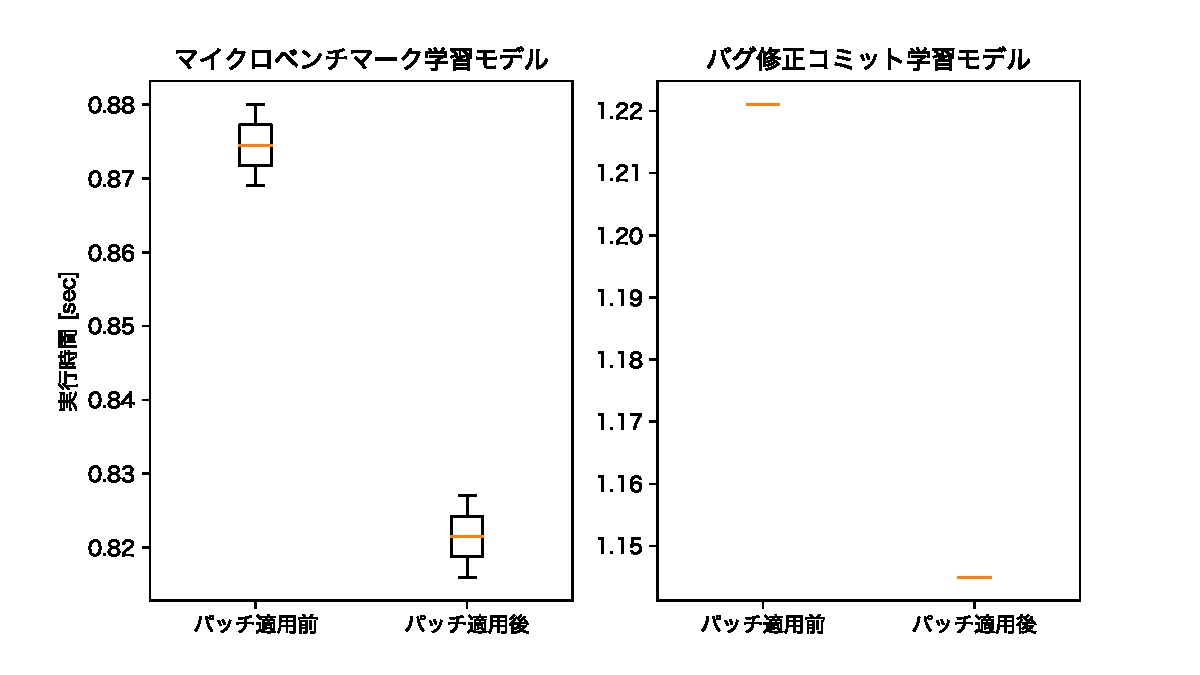
\includegraphics[width=0.85\linewidth]{figure/speed_up_boxplot.pdf}
\vspace{-4mm}
\caption{実行時間短縮パッチの平均実行時間の分布}

\label{figure:execution speed up}
\end{figure}


\begin{figure}[t]
\centering
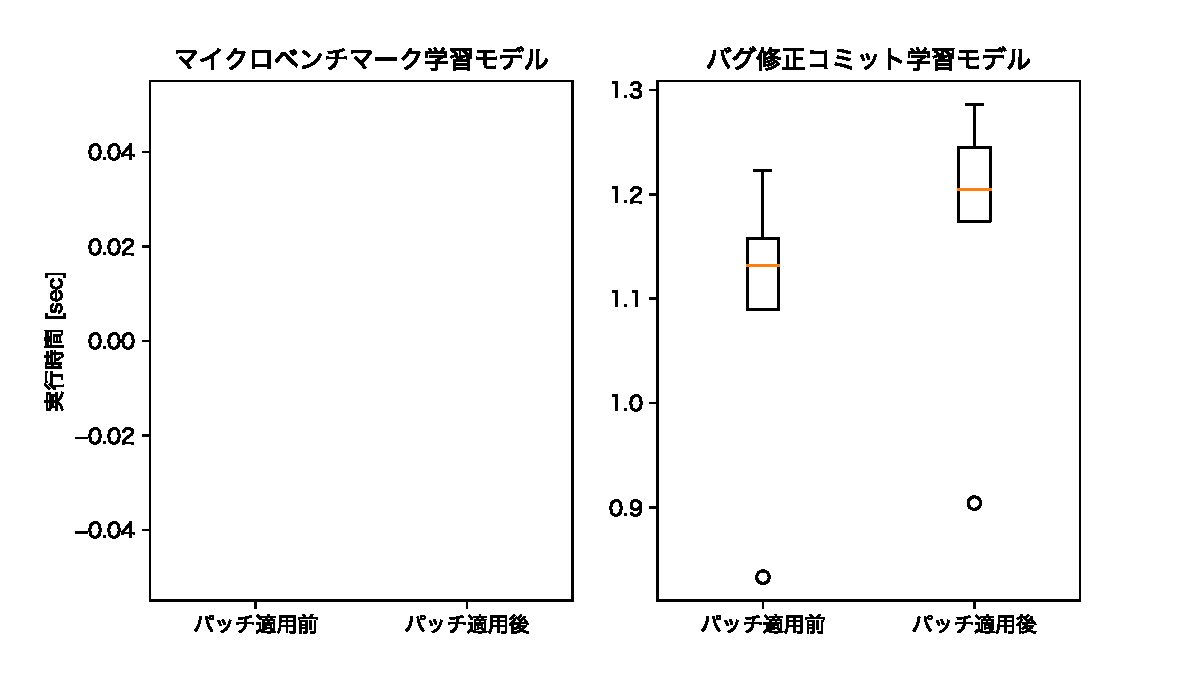
\includegraphics[width=0.85\linewidth]{figure/speed_down_boxplot.pdf}
\vspace{-4mm}
\caption{実行時間増加パッチの平均実行時間の分布\\(マイクロベンチマーク学習モデルは該当パッチなし)}
\vspace{-5mm}
\label{figure:execution speed down}
\end{figure}


図\ref{figure:execution speed up}および図\ref{figure:execution speed down}にパッチ適用前後で平均実行時間に有意差がみられたパッチの平均実行時間の分布を示す.図\ref{figure:execution speed up}から,約0.05秒平均実行時間を短縮したことが分かる.また,図\ref{figure:execution speed down}から,バグ修正コミット学習モデルが生成したパッチの中には,約0.05秒平均実行時間を増加させるパッチがあることが分かる.


テストスイートに通過したプログラム例をプログラム\ref{list:rq2 input1}〜\ref{list:rq2 patch2}に示す.


\listingcaption{実行時間を短縮させたプログラム例(入力プログラム)}
\begin{lstlisting}[label=list:rq2 input1]
errors.add('the value of ' + key + ' must be an integer', keyPath);
\end{lstlisting}

\listingcaption{実行時間を短縮させたプログラム例(生成パッチ)}
\begin{lstlisting}[label=list:rq2 patch1]
['the value of ', key].includes(key);
\end{lstlisting}


プログラム\ref{list:rq2 patch1}はマイクロベンチマーク学習モデルがプログラム\ref{list:rq2 input1}に対して生成し,テストを通過したパッチであるが,両プログラムの機能は異なる.プログラム\ref{list:rq2 input1}がオブジェクトerrorsに文字列を追加するプログラムであるのに対し,プログラム\ref{list:rq2 patch1}はincludes()メソッドを用いて配列内に変数keyが含まれるか判定しており,trueに判定される式を生成している.


\listingcaption{実行時間を増加させたプログラム例(入力プログラム)}
\begin{lstlisting}[label=list:rq2 input2]
var converted;
\end{lstlisting}

\listingcaption{実行時間を増加させたプログラム例(生成パッチ)}
\begin{lstlisting}[label=list:rq2 patch2]
var base = null ;
\end{lstlisting}


プログラム\ref{list:rq2 patch2}はバグ修正コミット学習モデルがプログラム\ref{list:rq2 input2}に対して生成し,テストを通過したパッチであるが,両プログラムは宣言する変数名が異なる.プログラム\ref{list:rq2 patch2}は変数の宣言と同時にnull値で初期化しているため,実行時間が増加したと考えられる.

%\subsubsection{まとめ}
%
%マイクロベンチマーク学習モデルは,バグ修正コミット学習モデルよりも1件多い,300件中2件の入力プログラムに対して実行速度を改善し,実行速度を低下させるパッチは0件だった.また,修正パッチを適用することで約0.05秒テストスイート実行時間を短縮した.


%%%%%%%%%%%%%%%
%\section{考察}\label{sec:discussion}
%%%%%%%%%%%%%%%
%
%\subsection{テストスイートによる生成パッチの選別}
%マイクロベンチマークを学習データセットとした自動修正モデルは,従来研究のバグ修正コミットをデータセットとしたモデルよりも多くの入力プログラムに対してテストを通過するパッチを生成できた.マイクロベンチマークは同一機能の実装方法を比較するプログラムであり,バグ修正コミットよりも入力プログラムの動作を損ねない変更方法を学習できることが示唆される.
%
%一方で,テストスイートを通過したプログラムはすべて入力プログラムと機能的に異なるプログラムであり,テストスイートを用いて機能的に異なるプログラムを除外することは困難であると考えられる.特に,JavaScriptの言語設計上,変数の宣言文を削除しても実行時エラーにならないため,提案手法による宣言文の自動修正は困難であることが分かった.
%
%\subsection{修正パッチによる実行速度改善}
%
%マイクロベンチマークを学習データセットとした自動修正モデルは,従来研究のバグ修正コミットをデータセットとしたモデルよりも多くの入力プログラムに対して実行速度を改善するパッチを生成し,修正パッチによって平均実行時間が約0.05秒短縮した.マイクロベンチマーク共有サービスを活用した学習モデルは,従来研究で提案されたバグ修正コミットを学習データセットに用いた自動修正モデルよりも実行速度改善性能が高いと考えられる.

%\subsection{妥当性への脅威}
%
%\subsubsection{内的妥当性}
%
%本研究では修正パッチによる実行時間の変化をテストスイートの実行時間を用いて比較している.実際のソフトウェア利用時には関数の呼出し回数が異なる等の理由で各プログラム行が全体の実行時間に与える影響がテストスイートとは異なる可能性が考えられる.
%
%\subsubsection{外的妥当性}
%
%本研究では評価データセットとしてGitHubコミットから追加行数が1行のみのプログラム変更断片を収集したため,連続する2行以上が変更されているプログラム断片に対しての提案モデルの性能は測定していない.したがって,if文やfor文等の他行と同時に追加されやすいプログラム行が評価データセットに出現しにくい等,評価データセット内のプログラムと実際の開発プログラムで頻繁に出現するプログラムとは異なる可能性が考えられる.

%%%%%%%%%%%%
\section{おわりに}\label{sec:conclusion}
%%%%%%%%%%%%

本研究では,マイクロベンチマーク共有サービスMeasureThat.netから収集した評価結果を学習データセットとしたニューラル機械翻訳モデルを用いて,実行速度の改善に特化したプログラム自動修正モデルを提案した.事前実験において,本研究で生成したモデルは58.66\%〜75.63\%の精度で実行速度を改善するプログラムを生成することができた.しかし,GitHubで公開されるプログラムを対象に高速化修正パッチの自動生成を試みたが,テストスイートを通過したプログラムは大半が入力プログラムと機能的に異なるプログラムであり,学習データセット数の少なさやJavaScript言語仕様上のテストスイートによる検証の難しさ等の課題があることが明らかになった.今後は,学習データセットを増やす等の改善を行うことで,より多くの入力プログラムに対して実行時間を短縮するプログラム修正パッチを生成できるようにすることができると考えられる.


%提案モデルが300件中19件の入力プログラムに対してテストスイートに通過する修正パッチを生成でき,2件の入力プログラムに対して実行時間を短縮できることを明らかにした.提案モデルが時間短縮に成功したプログラム件数は従来研究で用いられたバグ修正コミットを学習データセットに用いた自動修正モデルよりも多く,マイクロベンチマークを学習データセットにすることで実行速度改善性能が高いと考えられる.一方で,





\begin{acknowledgment}
ほげ
\end{acknowledgment}



\bibliographystyle{ipsjunsrt}

\bibliography{bibfile}


\end{document}
